\documentclass[aspectratio=169]{beamer}

\mode<presentation>

\usepackage[utf8]{inputenc}
\usepackage[T1]{fontenc}	%makes å,ä,ö etc. proper symbols
\usepackage{amsmath}
\usepackage{graphicx}
\usepackage{xcolor}
\usepackage{listings}
\usepackage{multicol}
\usepackage{hyperref}

\usepackage{animate}

\definecolor{LundaGroen}{RGB}{00,68,71}
\definecolor{StabilaLila}{RGB}{85,19,78}
\definecolor{VarmOrange}{RGB}{237,104,63}

\definecolor{MagnoliaRosa}{RGB}{251,214,209}
\definecolor{LundaHimmel}{RGB}{204,225,225}
\definecolor{LundaLjus}{RGB}{255,242,191}

\usefonttheme{serif}
\usetheme{malmoe}
\setbeamercolor{palette primary}{bg=VarmOrange}
\setbeamercolor{palette quaternary}{bg=LundaGroen}
\setbeamercolor{background canvas}{bg=LundaLjus}
\setbeamercolor{structure}{fg=LundaGroen}

\usepackage[many]{tcolorbox}

\newtcolorbox{cross}{blank,breakable,parbox=false,
  overlay={\draw[red,line width=5pt] (interior.south west)--(interior.north east);
    \draw[red,line width=5pt] (interior.north west)--(interior.south east);}}

\lstset{language=[LaTeX]Tex,%C++,
    morekeywords={PassOptionsToPackage,selectlanguage},
    keywordstyle=\color{blue},%\bfseries,
    basicstyle=\small\ttfamily,
    %identifierstyle=\color{NavyBlue},
    commentstyle=\color{red}\ttfamily,
    stringstyle=\color{orange},
    numbers=left,%
    numberstyle=\scriptsize,%\tiny
    stepnumber=1,
    numbersep=8pt,
    showstringspaces=false,
    breaklines=true,
    %frameround=ftff,
    frame=single,
    belowcaptionskip=.75\baselineskip,
	tabsize=4
    %frame=L
}
\lstset{language=Python} 
\lstset{backgroundcolor=\color{white}}

\newcounter{uppgifter}

\begin{document}

\lstset{literate=
  {á}{{\'a}}1 {é}{{\'e}}1 {í}{{\'i}}1 {ó}{{\'o}}1 {ú}{{\'u}}1
  {Á}{{\'A}}1 {É}{{\'E}}1 {Í}{{\'I}}1 {Ó}{{\'O}}1 {Ú}{{\'U}}1
  {à}{{\`a}}1 {è}{{\`e}}1 {ì}{{\`i}}1 {ò}{{\`o}}1 {ù}{{\`u}}1
  {À}{{\`A}}1 {È}{{\'E}}1 {Ì}{{\`I}}1 {Ò}{{\`O}}1 {Ù}{{\`U}}1
  {ä}{{\"a}}1 {ë}{{\"e}}1 {ï}{{\"i}}1 {ö}{{\"o}}1 {ü}{{\"u}}1
  {Ä}{{\"A}}1 {Ë}{{\"E}}1 {Ï}{{\"I}}1 {Ö}{{\"O}}1 {Ü}{{\"U}}1
  {â}{{\^a}}1 {ê}{{\^e}}1 {î}{{\^i}}1 {ô}{{\^o}}1 {û}{{\^u}}1
  {Â}{{\^A}}1 {Ê}{{\^E}}1 {Î}{{\^I}}1 {Ô}{{\^O}}1 {Û}{{\^U}}1
  {œ}{{\oe}}1 {Œ}{{\OE}}1 {æ}{{\ae}}1 {Æ}{{\AE}}1 {ß}{{\ss}}1
  {ű}{{\H{u}}}1 {Ű}{{\H{U}}}1 {ő}{{\H{o}}}1 {Ő}{{\H{O}}}1
  {ç}{{\c c}}1 {Ç}{{\c C}}1 {ø}{{\o}}1 {å}{{\r a}}1 {Å}{{\r A}}1
  {€}{{\euro}}1 {£}{{\pounds}}1 {«}{{\guillemotleft}}1
  {»}{{\guillemotright}}1 {ñ}{{\~n}}1 {Ñ}{{\~N}}1 {¿}{{?`}}1
}

\lstset{escapeinside={(*@}{@*)}}

% NEW COMMANDS
\AtBeginSection[ ]
{
\begin{frame}{Outline}
\setbeamercolor{section in toc shaded}{fg=LundaGroen}
\setbeamercolor{subsection in toc shaded}{fg=black}
    \tableofcontents[currentsection]

\end{frame}
}

\title{Grafer}
\date{vt 24}
\author{Programmering 2}

\maketitle

\section{Grafer}

\subsection{Repetition}

\begin{frame}[fragile]
	\frametitle{Repetition}
	
	\begin{lstlisting}
from matplotlib import pyplot as plt
import numpy as np

x_data = np.linspace(-np.pi, np.pi, 10) # Skapar tio tal mellan -pi och pi
y_data = [np.sin(x) for x in x_data] # En sinus-kurva

plt.plot(x_data, y_data, '.')
plt.show()
	\end{lstlisting}

\end{frame}

\subsection{Nyheter}

\begin{frame}
	\frametitle{Annoteringar}
	
	\centering
	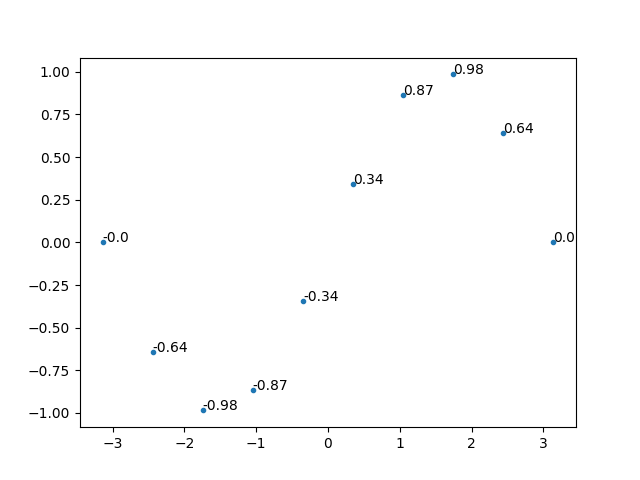
\includegraphics[width=.65\linewidth]{Figure-1.png}
	
\end{frame}

\begin{frame}[fragile]
	\frametitle{Annoteringar}

	\begin{lstlisting}
from matplotlib import pyplot as plt
import numpy as np

x_data = np.linspace(-np.pi, np.pi, 10) # Skapar tio tal mellan -pi och pi
y_data = [np.sin(x) for x in x_data] # En sinus-kurva

plt.plot(x_data, y_data, '.')

for i in range(len(y_data)):
    # Labels
    plt.annotate(round(y_data,2), (x_data[i], y_data[i])) 
    
plt.show()
	\end{lstlisting}
	
\end{frame}

\section{Uppdaterande graf}

\begin{frame}[fragile]
	\frametitle{Uppdaterande graf}
	
	\begin{itemize}
		\item Det finns ett par olika sätt att uppdatera en graf
			\begin{itemize}
				\item Uppdatera redan existerande värden
				\item Lägga till nya värden
		\end{itemize}
		\item Båda kräver samma funktion \lstinline{plt.ion()}
		\item Vi behöver också använda fler objekt
	\end{itemize}
	
\end{frame}

\begin{frame}[fragile]

	\begin{itemize}
		\item För att ha en interaktiv graf behöver vi ha mer kontroll över grafen
		\item Det får vi genom att använda figurer
	\end{itemize}
	
	\begin{lstlisting}
from matplotlib import pyplot as plt
import numpy as np

x_data = np.linspace(-np.pi, np.pi, 100)
y_data = [np.sin(x) for x in x_data]

fig = plt.figure() # Skapar en figur (typ fönstret)
ax = fig.add_subplot(111) # Lägger till ett ritområde
ax.plot(x_data, y_data) # Rita grafen
fig.show() # Visa fönstret med grafen
	\end{lstlisting}

\end{frame}

\subsection{Uppdatera värden}

\begin{frame}[fragile]
	\frametitle{Uppdatera värden}
	
	\begin{lstlisting}
fig = plt.figure() # Skapar en figur (typ fönstret)
ax = fig.add_subplot(111) # Lägger till ett ritområde
ax.plot(x_data, y_data) # Rita grafen
# Skapa ny data
ny_y = np.array([np.cos(x) for x in x_data])
line = ax.get_lines()[0] # Hämta första ritade linjen
line.set_ydata(ny_y)
fig.show()
	\end{lstlisting}
	
\end{frame}

\begin{frame}
	\frametitle{Uppdaterande graf}
	
	\centering
	\animategraphics[loop,controls,width=.5\linewidth]{10}{loop-}{1}{20}
	
\end{frame}

\begin{frame}[fragile]
	\frametitle{Se förändringarna}
	
	\begin{lstlisting}
plt.ion()
fig = plt.figure() # Skapar en figur (typ fönstret)
ax = fig.add_subplot(111) # Lägger till ett ritområde
ax.plot(x_data, y_data) # Rita grafen
line = ax.get_lines()[0]
fig.show() # Visa fönstret med grafen
t = 0
while True:
    t += np.pi/10 # Förskjutningen
    line.set_ydata(np.array([np.sin(x+t) for x in x_data]))
    fig.canvas.draw() # Ritar ut
	\end{lstlisting}
	
\end{frame}

\subsection{Lägg till nya värden}

\begin{frame}
	\frametitle{Graf med nya värden}
	
	\centering
	\animategraphics[loop,controls,width=.5\linewidth]{10}{append-}{1}{20}
	
\end{frame}

\begin{frame}[fragile]
	\frametitle{Se förändringarna}
	
	\begin{lstlisting}
plt.ion()
fig = plt.figure() # Skapar en figur (typ fönstret)
ax = fig.add_subplot(111) # Lägger till ett ritområde
ax.plot(x_data, y_data) # Rita grafen
line = ax.get_lines()[0]
fig.show() # Visa fönstret med grafen
t = np.pi
while i < 100:
    t += np.pi/10
    x_data = np.append(x_data, t) # Arrayer är besvärliga
    line.set_xdata(x_data) # Uppdatera x_data, nästa rad y_data
    line.set_ydata(np.array([np.sin(x) for x in x_data]))
    ax.set_autoscaley_on(True) # Behövs inte för exemplet
    ax.set_xlim(min(x_data), max(x_data))
    fig.canvas.draw()
	\end{lstlisting}
	
\end{frame}

\section{Övningar}

\begin{frame}
	\frametitle{Övningar}
	
	\begin{enumerate}
		\item Återskapa graferna från övningarna
		\item Annotera alla graferna
		\item Prata med Calle för fler övningar
	\end{enumerate}

\end{frame}


\end{document}